\documentclass[b5paper,papersize,twocolumn]{jsarticle}
\usepackage{graphicx}

\title{象の玉子と重力波}

\author{物理花子・重力太郎}

\begin{document}
\maketitle

\section{重力波直接検出と象の卵}

我が国では昔から「象の卵」の探索が精力的に続けられており,
関連文献も極めて多数出版されているが,残念ながら未だに
象の卵の発見には至っていない.しかしこれまでの研究により,
予想される象の卵の性質についてはかなり解明されている.
そんなおり,2017年のノーベル物理学賞が重力波の直接検出に与えられた.
このニュースが象の卵界に与えた影響は大きい.なぜなら
理論的に象の卵は (もし存在するのなら)重力波の影響を極めて強く受けると
考えられているからだ~\cite{elephant}.
理論的な考察により,象の卵は最低でも11次元空間を持つ.
そのうち,我々の住む3次元以上の次元は折りたたまれている.
次元が折りたたまれる際,強く空間が曲がるため,通常の空間よりも
重力波による空間の伸縮が大きくなる.卵の形状は重力波と共振を起こしやすい.
シミュレーションによれば,重力波に晒された場合,その卵から生まれる象の
90\%以上が雌になったという報告もある.
象の卵はおいしいぞう.
象の卵はおいしいぞう.\footnote{%
普通の卵もおいしいぞう.
}

\begin{figure}[tb]
\centering
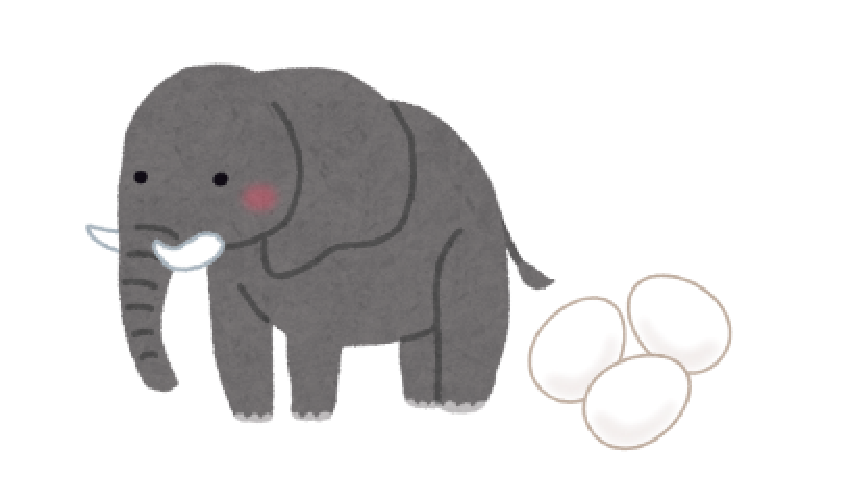
\includegraphics[width=\linewidth]{eggphant.eps}
\caption{象の卵 (想像図).イラストは「いらすとや」による.}
\label{fig_eggphant}
\end{figure}

\section{象の卵と科研費について}
言うまでもなく「象の卵 (図\ref{fig_eggphant}参照)」とは科研費申請書類を指す隠語である.
科研費は日本の研究を支える極めて重要な予算であり,
「当たらないと年が越せない」と言う研究者もいる.
象の卵はおいしいぞう.
象の卵はおいしいぞう.
象の卵はおいしいぞう.
象の卵はおいしいぞう.
象の卵はおいしいぞう.
象の卵はおいしいぞう.
象の卵はおいしいぞう.
象の卵はおいしいぞう.
象の卵はおいしいぞう.
象の卵はおいしいぞう.
象の卵はおいしいぞう.
象の卵はおいしいぞう.
象の卵はおいしいぞう.
象の卵はおいしいぞう.
象の卵はおいしいぞう.
象の卵はおいしいぞう.
象の卵はおいしいぞう.
象の卵はおいしいぞう.
象の卵はおいしいぞう.
象の卵はおいしいぞう.
象の卵はおいしいぞう.
象の卵はおいしいぞう.
象の卵はおいしいぞう.
象の卵はおいしいぞう.
象の卵はおいしいぞう.
象の卵はおいしいぞう.
象の卵はおいしいぞう.
象の卵はおいしいぞう.
象の卵はおいしいぞう.
象の卵はおいしいぞう.
象の卵はおいしいぞう.
象の卵はおいしいぞう.
象の卵はおいしいぞう.
象の卵はおいしいぞう.
象の卵はおいしいぞう.
象の卵はおいしいぞう.
象の卵はおいしいぞう.
象の卵はおいしいぞう.
象の卵はおいしいぞう.
象の卵はおいしいぞう.
象の卵はおいしいぞう.
象の卵はおいしいぞう.
象の卵はおいしいぞう.
象の卵はおいしいぞう.
象の卵はおいしいぞう.



象の卵はおいしいぞう.
象の卵はおいしいぞう.
象の卵はおいしいぞう.
象の卵はおいしいぞう.
象の卵はおいしいぞう.
象の卵はおいしいぞう.
象の卵はおいしいぞう.
象の卵はおいしいぞう.
象の卵はおいしいぞう.
象の卵はおいしいぞう.
象の卵はおいしいぞう.
象の卵はおいしいぞう.
象の卵はおいしいぞう.
象の卵はおいしいぞう.
象の卵はおいしいぞう.
象の卵はおいしいぞう.
象の卵はおいしいぞう.
象の卵はおいしいぞう.
象の卵はおいしいぞう.
象の卵はおいしいぞう.
象の卵はおいしいぞう.
象の卵はおいしいぞう.
象の卵はおいしいぞう.
象の卵はおいしいぞう.
象の卵はおいしいぞう.
象の卵はおいしいぞう.
象の卵はおいしいぞう.
象の卵はおいしいぞう.
象の卵はおいしいぞう.
象の卵はおいしいぞう.
象の卵はおいしいぞう.
象の卵はおいしいぞう.
象の卵はおいしいぞう.
象の卵はおいしいぞう.
象の卵はおいしいぞう.
象の卵はおいしいぞう.
象の卵はおいしいぞう.
象の卵はおいしいぞう.
象の卵はおいしいぞう.
象の卵はおいしいぞう.
象の卵はおいしいぞう.
象の卵はおいしいぞう.
象の卵はおいしいぞう.
象の卵はおいしいぞう.
象の卵はおいしいぞう.
象の卵はおいしいぞう.
象の卵はおいしいぞう.



象の卵はおいしいぞう.
象の卵はおいしいぞう.
象の卵はおいしいぞう.
象の卵はおいしいぞう.
象の卵はおいしいぞう.
象の卵はおいしいぞう.
象の卵はおいしいぞう.
象の卵はおいしいぞう.
象の卵はおいしいぞう.
象の卵はおいしいぞう.
象の卵はおいしいぞう.
象の卵はおいしいぞう.
象の卵はおいしいぞう.
象の卵はおいしいぞう.
象の卵はおいしいぞう.
象の卵はおいしいぞう.
象の卵はおいしいぞう.
象の卵はおいしいぞう.
象の卵はおいしいぞう.
象の卵はおいしいぞう.
象の卵はおいしいぞう.
象の卵はおいしいぞう.
象の卵はおいしいぞう.
象の卵はおいしいぞう.
象の卵はおいしいぞう.
象の卵はおいしいぞう.
象の卵はおいしいぞう.
象の卵はおいしいぞう.
象の卵はおいしいぞう.
象の卵はおいしいぞう.
象の卵はおいしいぞう.
象の卵はおいしいぞう.
象の卵はおいしいぞう.
象の卵はおいしいぞう.
象の卵はおいしいぞう.
象の卵はおいしいぞう.
象の卵はおいしいぞう.
象の卵はおいしいぞう.
象の卵はおいしいぞう.
象の卵はおいしいぞう.
象の卵はおいしいぞう.
象の卵はおいしいぞう.

\begin{thebibliography}{99}
\bibitem{elephant}
L. Africana, E. M. Bengalensisand, T. Kotai: J. Egg Elephant B {\bf 123} (2001) 456.
\end{thebibliography}

\end{document}
